\chapter{Miniprojekt 3}
\section{Opgavebeskrivelse}
Opgaven lyder på at lave et selvvalgt projekt, som skal indeholde væsentlige elementer fra hele kurset. \\
Med udgangspunkt i ovenstående, er der valgt en opgave som lyder på følgende: \\
Analyser og sammenligne relevante analyser via filtre og FFT.
Til analysen er valgt et simpelt lydsignal hvor hhv. en kvinde siger "hello" og en mand siger "hello".\\ \\
Opgaven er valgt ud fra teorien om, at hvis der er mange harmoniske overtoner og få eller meget svage disharmoniske overtoner, lyder stemmen meget ren. Hvis billedet derimod er præget af mange kraftige, disharmoniske overtoner lyder stemmen uren eller hæs.
\section{Analyse}
Først er der oprettet 3 filtre, et lavpas, båndpas og højpas filter, som gør sig gældende på begge signaler. Filtrenes knækfrekvenser er alle inden for det hørbarespektrum, eftersom analysen er af et hørbart lydsignal. Knækfrekvenserne er sat til:
\begin{itemize}
	\item Lavpas øvre = 7000
	\item Båndpas nedre = 6900
	\item Båndpas øvre = 14000
	\item Højpas nedre = 13900
\end{itemize}
\subsection{Filtrering}
Nedenfor, på figur \ref{Filtreret signal} ses det filtrerede signal for både man og dame:

\begin{figure}[H]
	\centering
	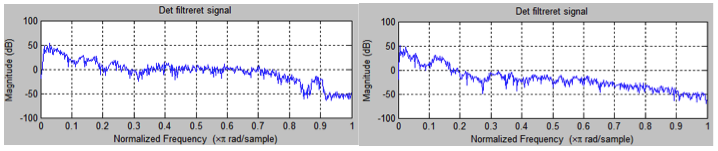
\includegraphics[width=1\textwidth]{Figurer/1}
	\label{Filtreret signal}
	\caption{Filtreret signal}
\end{figure}

\begin{figure}[H]
	\centering
	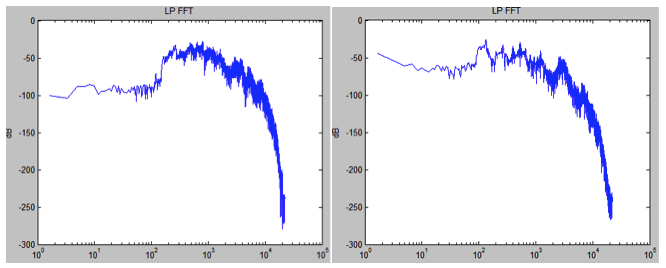
\includegraphics[width=1\textwidth]{Figurer/2}
	\label{FFT signal}
	\caption{FFT lavpas}
\end{figure}

\begin{figure}[H]
	\centering
	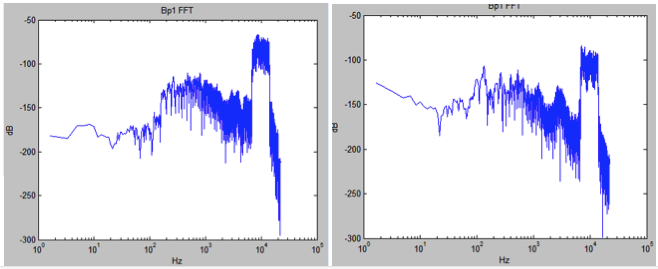
\includegraphics[width=1\textwidth]{Figurer/5}
	\label{FFT baandpas}
	\caption{FFT båndpas}
\end{figure}

\begin{figure}[H]
	\centering
	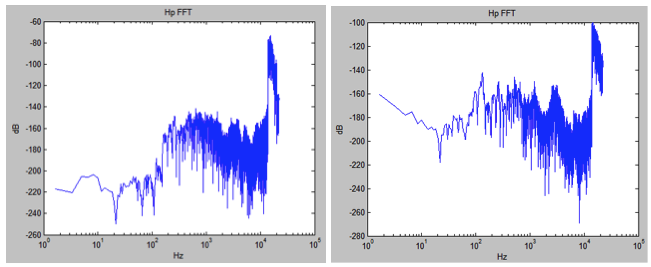
\includegraphics[width=1\textwidth]{Figurer/6}
	\label{FFT hoejpas}
	\caption{FFT højpas}
\end{figure}

\begin{figure}[H]
	\centering
	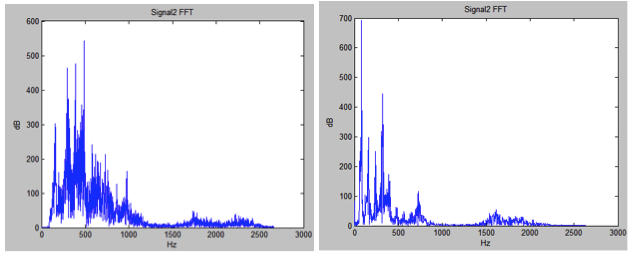
\includegraphics[width=1\textwidth]{Figurer/8}
	\label{FFT Signal}
	\caption{FFT Signal}
\end{figure}

\begin{figure}[H]
	\centering
	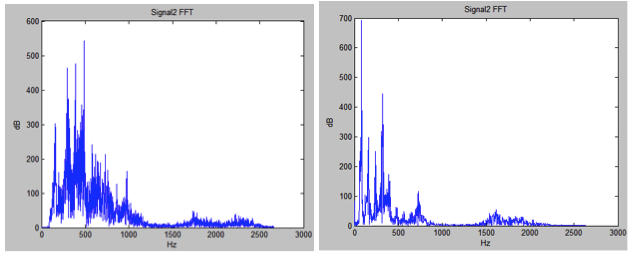
\includegraphics[width=1\textwidth]{Figurer/8}
	\label{Singalimpuls}
	\caption{Signalimpuls}
\end{figure}

\begin{figure}[H]
	\centering
	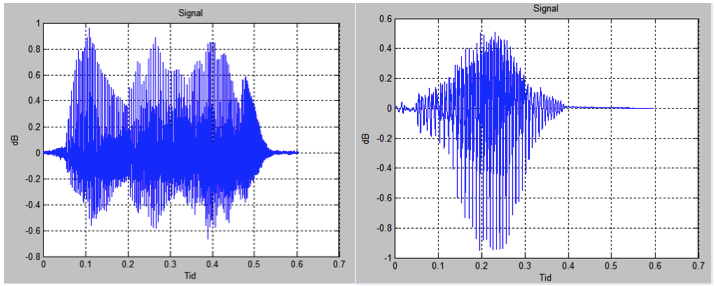
\includegraphics[width=1\textwidth]{Figurer/10}
	\label{Lyd}
	\caption{Lyd}
\end{figure}

\section{Konklusion}